\documentclass[9pt,a4paper]{article}
\usepackage[margin=0.7in]{geometry}
\usepackage{hyperref}
\usepackage[final]{pdfpages}
\usepackage{subcaption}

\title{A Title}

\author{Daniel Ramos \\ 81620 \and Miguel Tavares \\ 83528 \and Ricardo Brancas  \\ 83557}

\begin{document}
\maketitle

\section{Introduction}
The goal of this project is to analyse and characterize a real world network, and to  get 
acquainted with tools and methods which will be useful in following endeavours.
As such, we have chosen to analyse a snapshot of the Portuguese section of Wikipedia \cite{dataset};
we have chosen such a large network in order to get familiarized with tools such as Webgraph \cite{webgraph}.

To analyse our data we use Webgraph, including snippets of code made available
by Prof. Alexandre Francisco \cite{aplf}.

%TODO

\section{Methods}
The network was originally represented as an edge list which was subsequently converted in an adjacency list (ASCII Graph), by use of a simple \texttt{C++} program, as this is the input
format for Webgraph's compression algorithms.





\section{Results}
\subsection{Data summary}
Our network contains $1\,603\,222$ vertices and $49\,021\,409$ edges. Both the minimum in and out degrees are $0$, the maximum in degree is $207254$, and the maximum out degree is $12237$, finally the combined average degree of approximately $61.15$.

\subsection{Outras coisas}

In figure ~\ref{fig:inddist} we present the cumulative out degree distribution and ~\ref{fig:outddist}

\begin{figure}[h]
	\centering
	\begin{subfigure}{.5\textwidth}
		\centering
		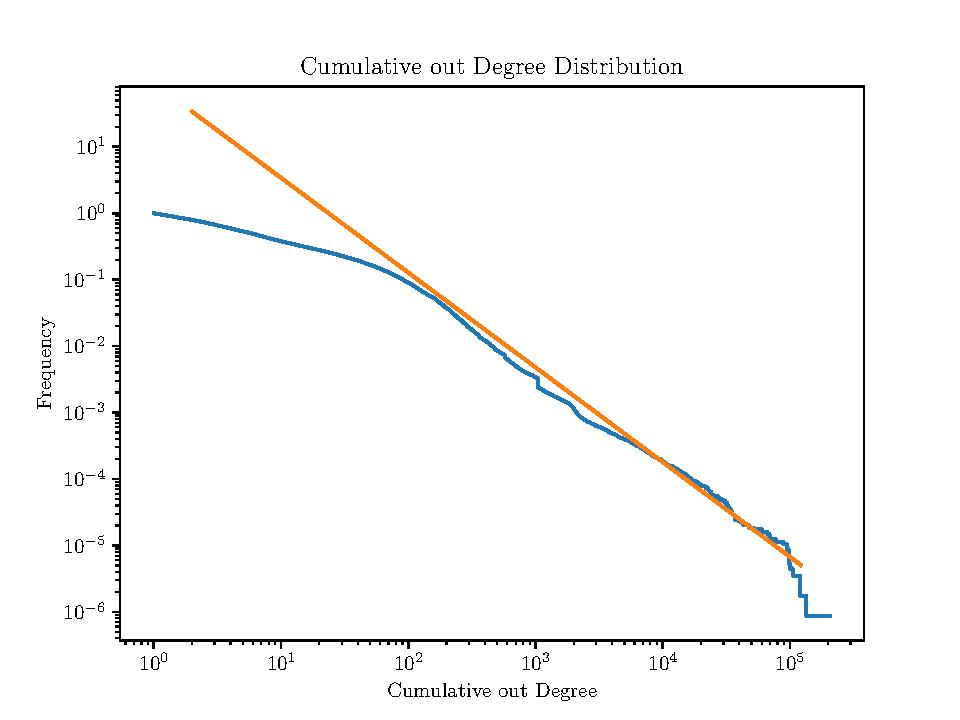
\includegraphics[width=\linewidth]{wikipedia_pt_in.pdf}
		\caption{Cumulative in-degree distribution.}
		\label{fig:inddist}
	\end{subfigure}%
	\begin{subfigure}{.5\textwidth}
		\centering
		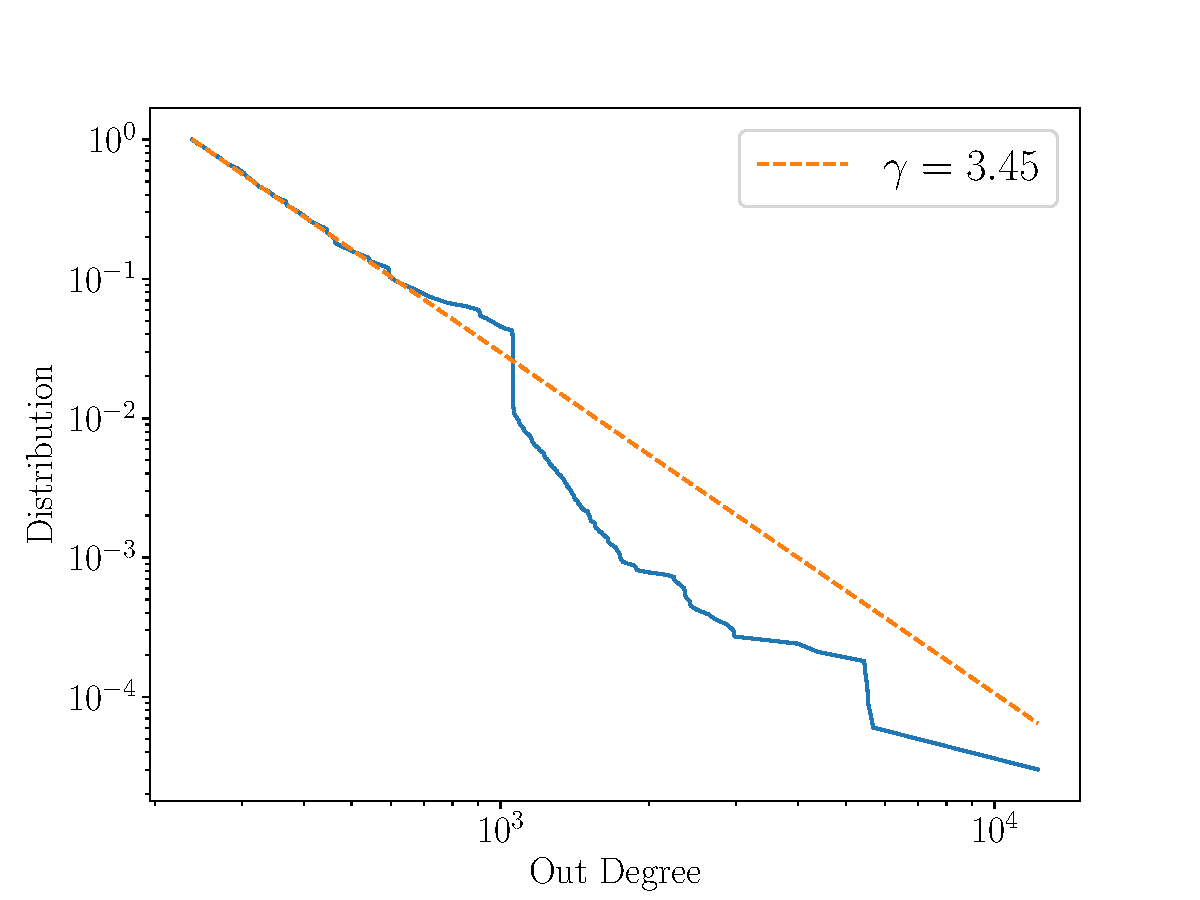
\includegraphics[width=\linewidth]{wikipedia_pt_out.pdf}
		\caption{Cumulative out-degree distribution.}
		\label{fig:outddist}
	\end{subfigure}
	\caption{Degree distributions.}
\end{figure}



\section{Discussion}

\begin{thebibliography}{9}
\bibitem{dataset}
Wikipedia links, portuguese network dataset -- KONECT, April 2017.
\\ \url{http://konect.uni-koblenz.de/networks/wikipedia\_link\_pt}

\bibitem{webgraph}
Webgraph
\\ \url{http://webgraph.di.unimi.it}

\bibitem{aplf}
A P Francisco: Webgraph related stuff
\\ \url{http://web.ist.utl.pt/aplf/code/webgraph}

\end{thebibliography}

\end{document}
